\clearpage
\begin{appendices}
  \label{transpiled_circuits}
  \clearpage

\begin{figure*}[h!]
  \centering
  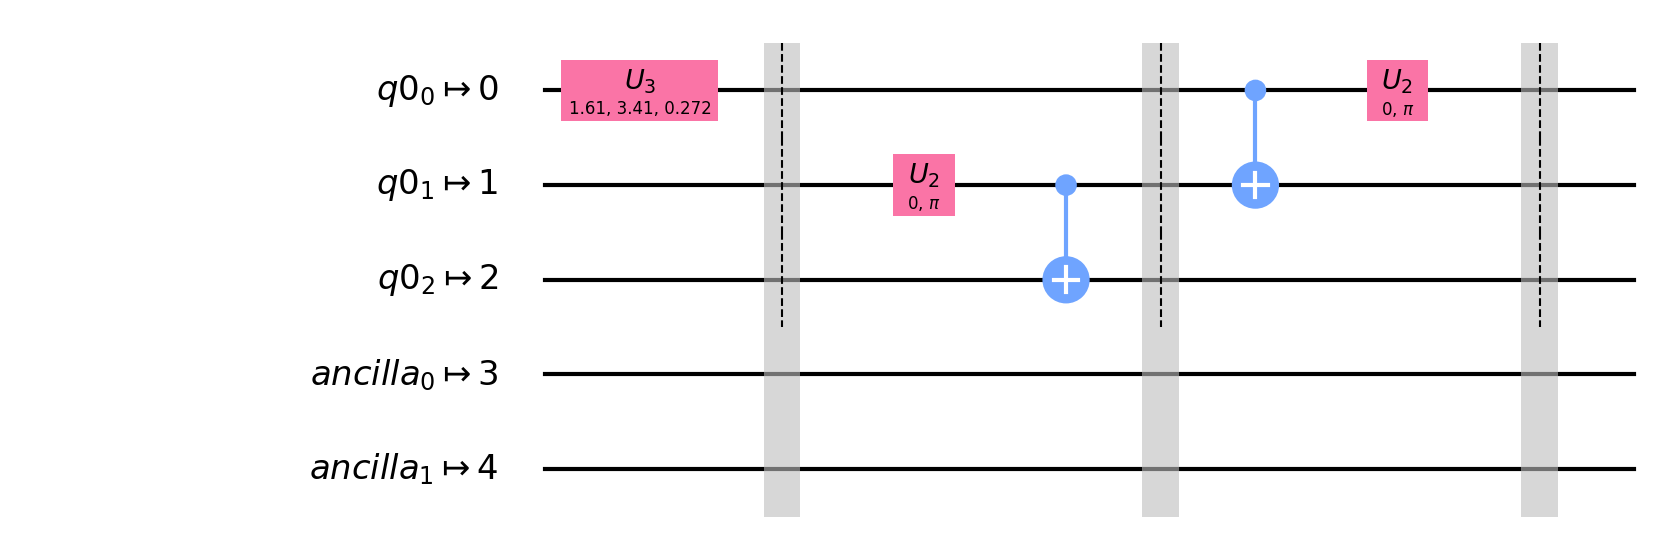
\includegraphics[width=0.8\textwidth]{images/teleport_ibmqx2.png}
  \caption{\textbf{Teleportation:} All backends implement the teleportation
    protocol with the same gate set. Variability between the three backends can
    therefore not be explained by different transpiling needs.}
  \label{fig:tele_trans}
\end{figure*}

% SWAPPING CIRCUITS
\begin{figure*}
  \centering
  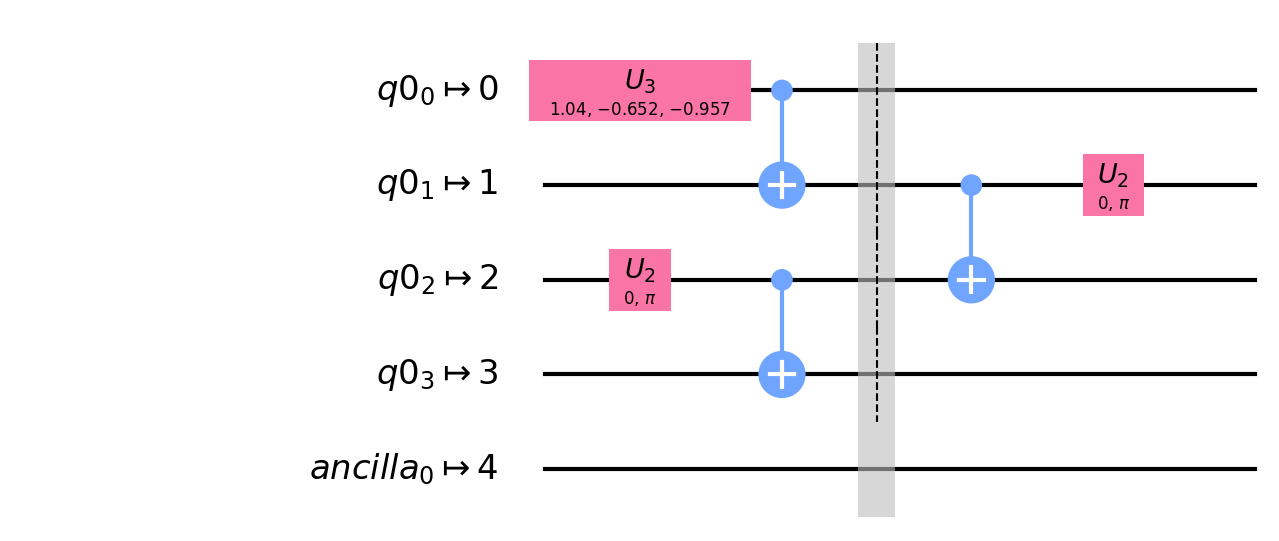
\includegraphics[width=0.6\textwidth]{images/swap_ibmqx2.png}
  \caption{\textbf{Entanglement swapping Yorktown:} Yorktown and Melbourne both
    implement swap with the minimal number of CNOT gates.}
  \label{fig:swap_york_trans}
\end{figure*}
  
\begin{figure*}
  \centering
  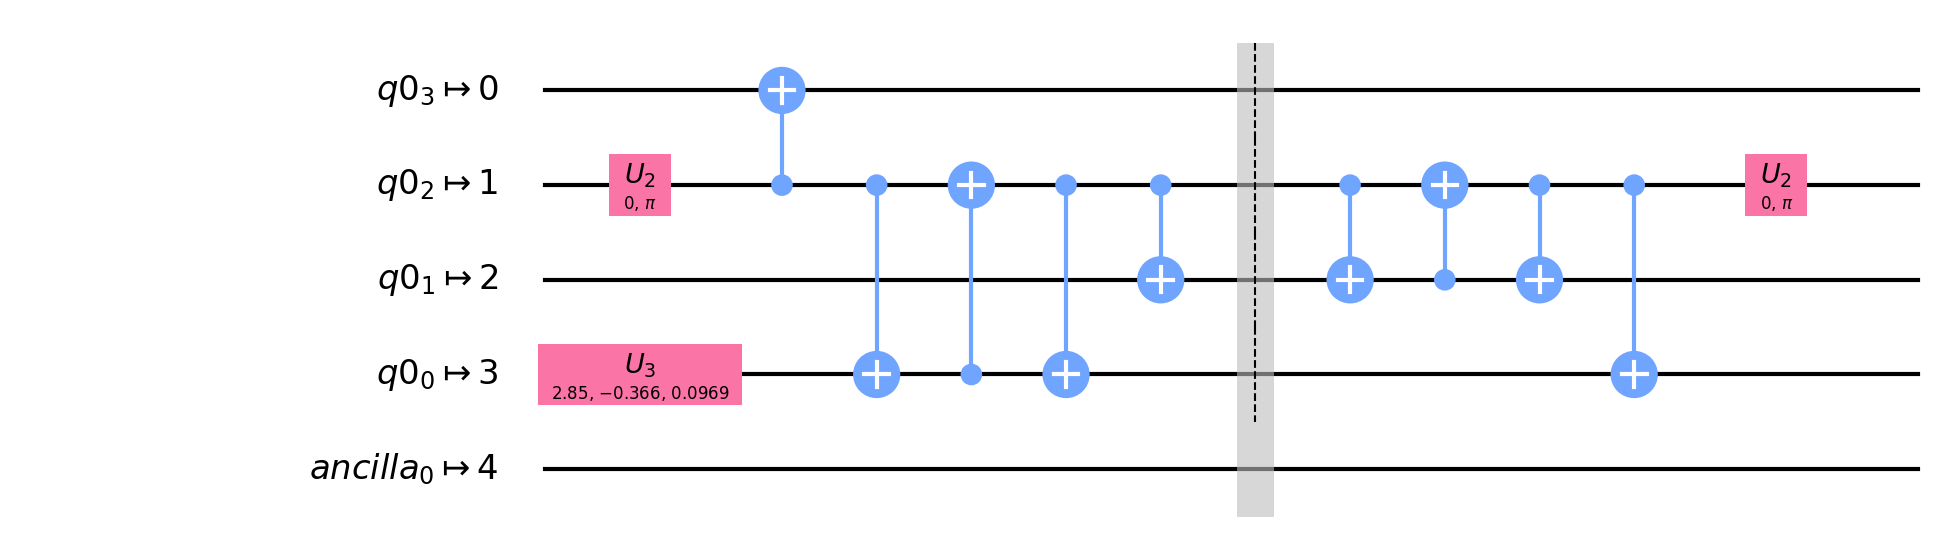
\includegraphics[width=\textwidth]{images/swap_burlington.png}
  \caption{\textbf{Entanglement swapping Burlington:} The Burlington backend
    requires three times as many CNOT gates to implement the swapping protocol,
    leading to drastically reduced output fidelities.}
  \label{fig:swap_burl_trans}
\end{figure*}

% PURIFICATION CIRCUITS
\begin{figure*}
  \centering
  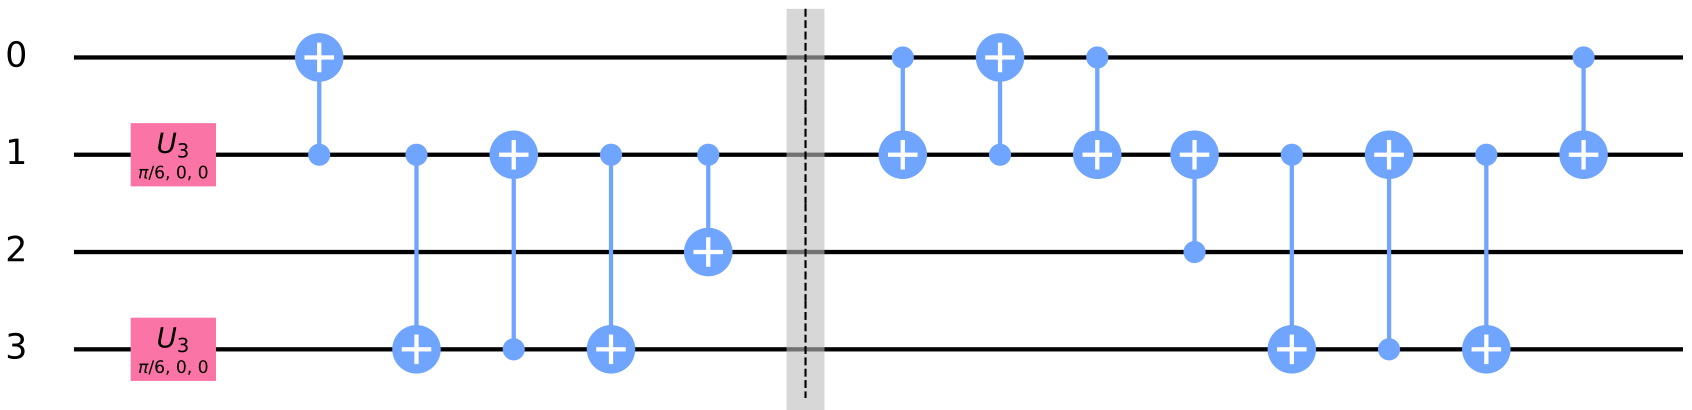
\includegraphics[width=\textwidth]{images/purification_burlington.png}
  \caption{\textbf{Purification protocol Burlington:} Each backend implements
    the purification protocol in a unique set of gates depending on the
    geometry. Burlington uses a total of 13 CNOT gates.}
  \label{fig:pur_burl_trans}
\end{figure*}

\begin{figure*}
  \centering
  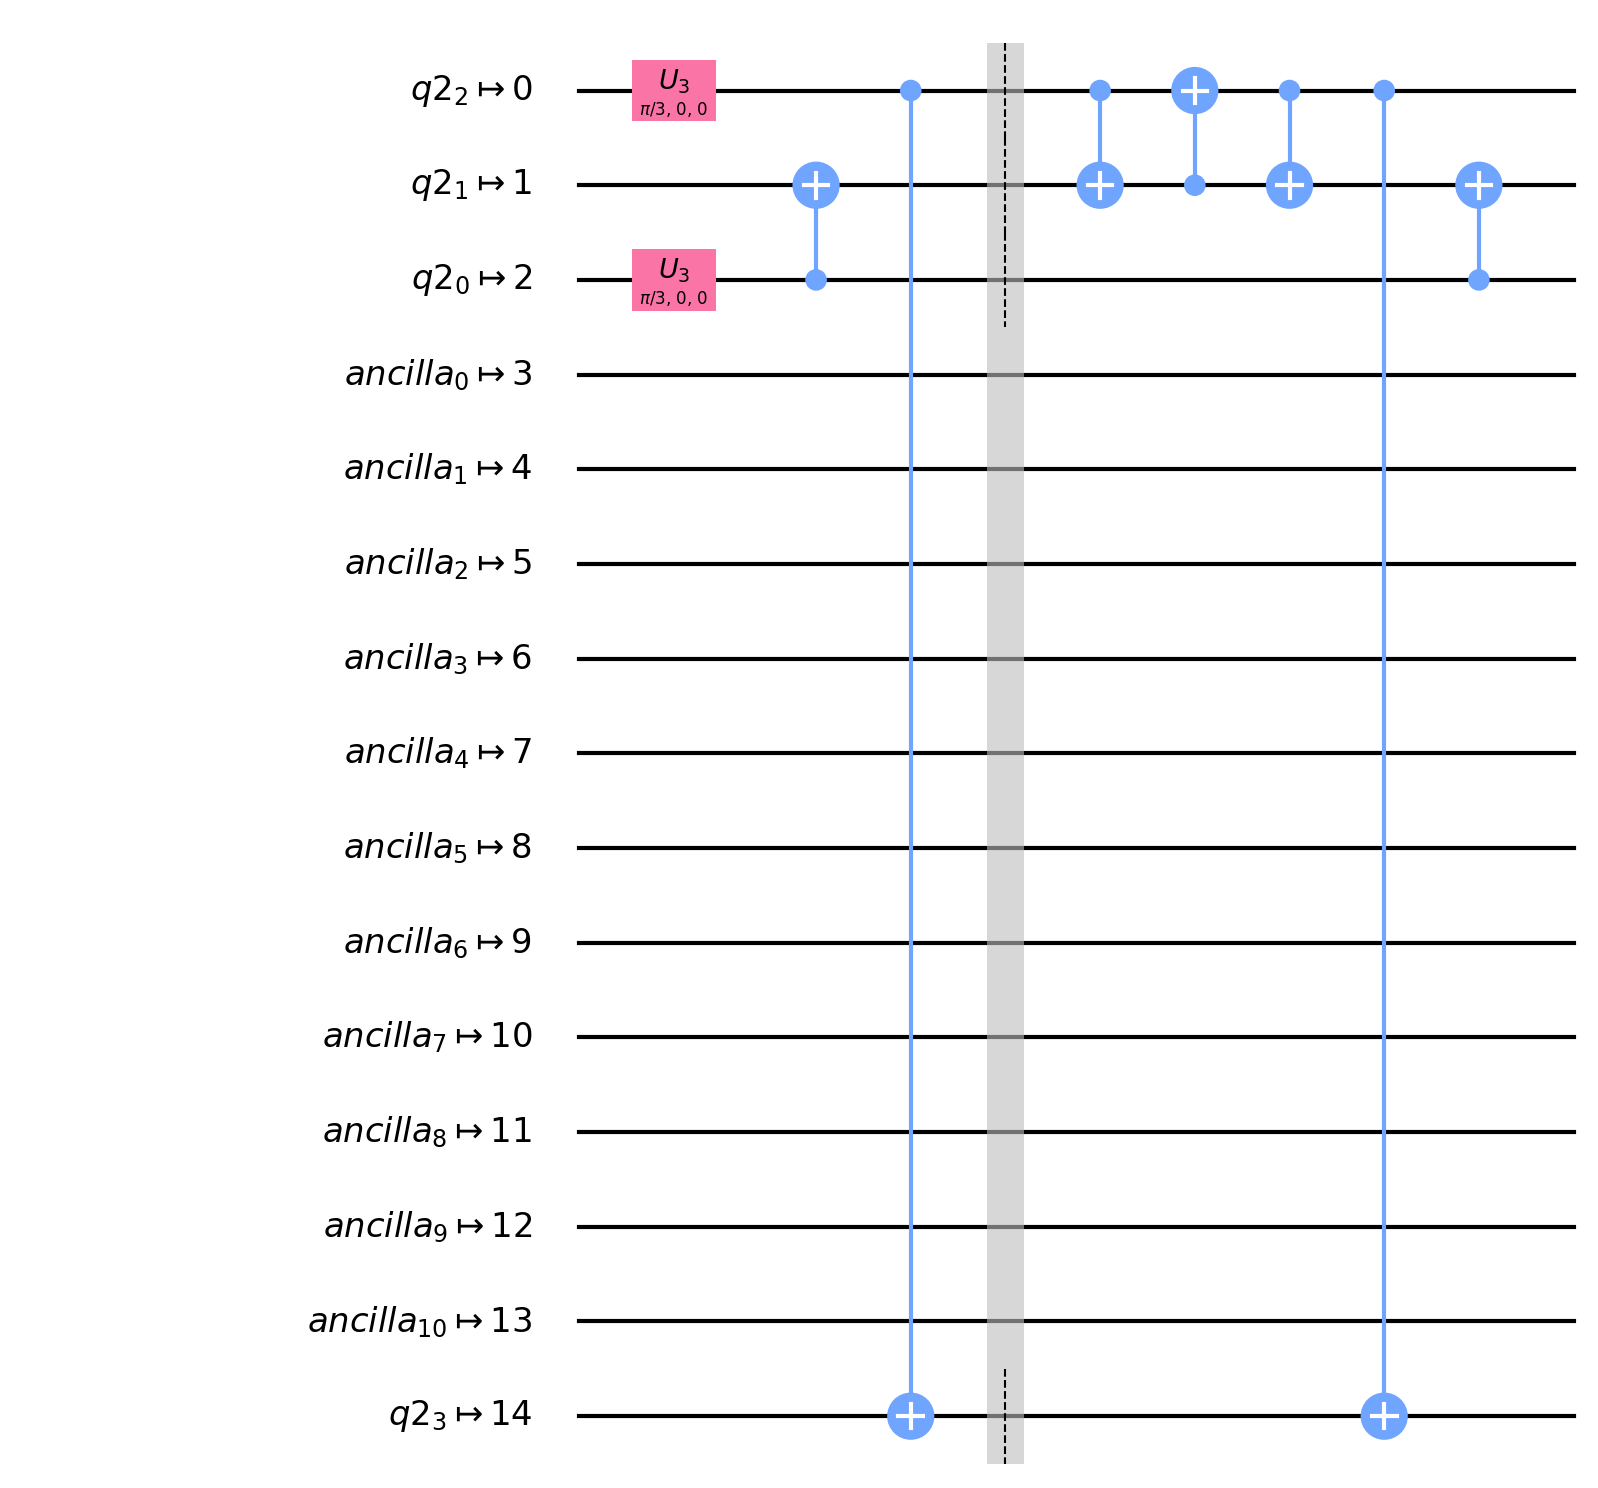
\includegraphics[height=0.3\textwidth]{images/purification_melbourne.png}
  \caption{\textbf{Purification protocol Melbourne:} Both Melbourne and Yorktown
    manage the purification protocol with just 7 CNOT gates, which may explain
    part of Burlington's poor performance compared to the other two backends.}
  \label{fig:pur_mel_trans}
\end{figure*}

\begin{figure*}
  \centering
  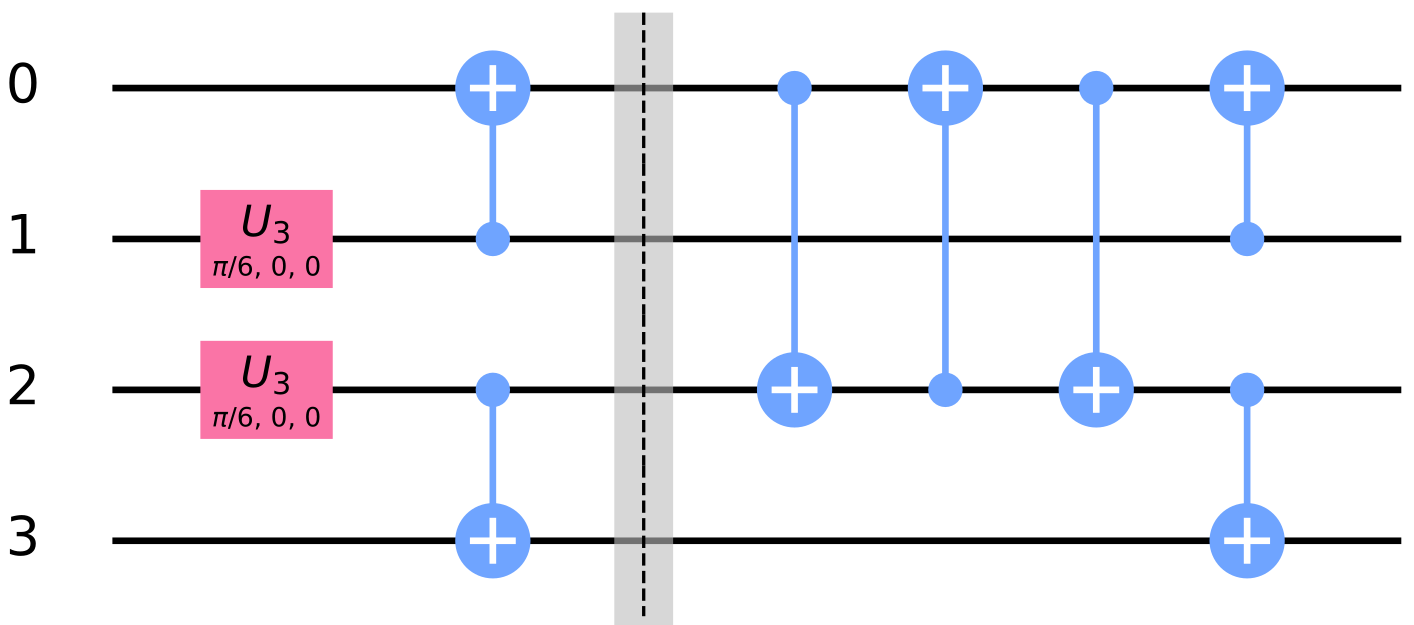
\includegraphics[height=0.3\textwidth]{images/purification_ibmqx2.png}
  \caption{\textbf{Purification protocol Yorktown:} The Yorktown backend uses 7
    CNOT gates to implement the circuit, almost half that of Burlington.}
  \label{fig:pur_york_trans}
\end{figure*}

% GROVER CIRCUIT
\begin{figure*}
  \centering
  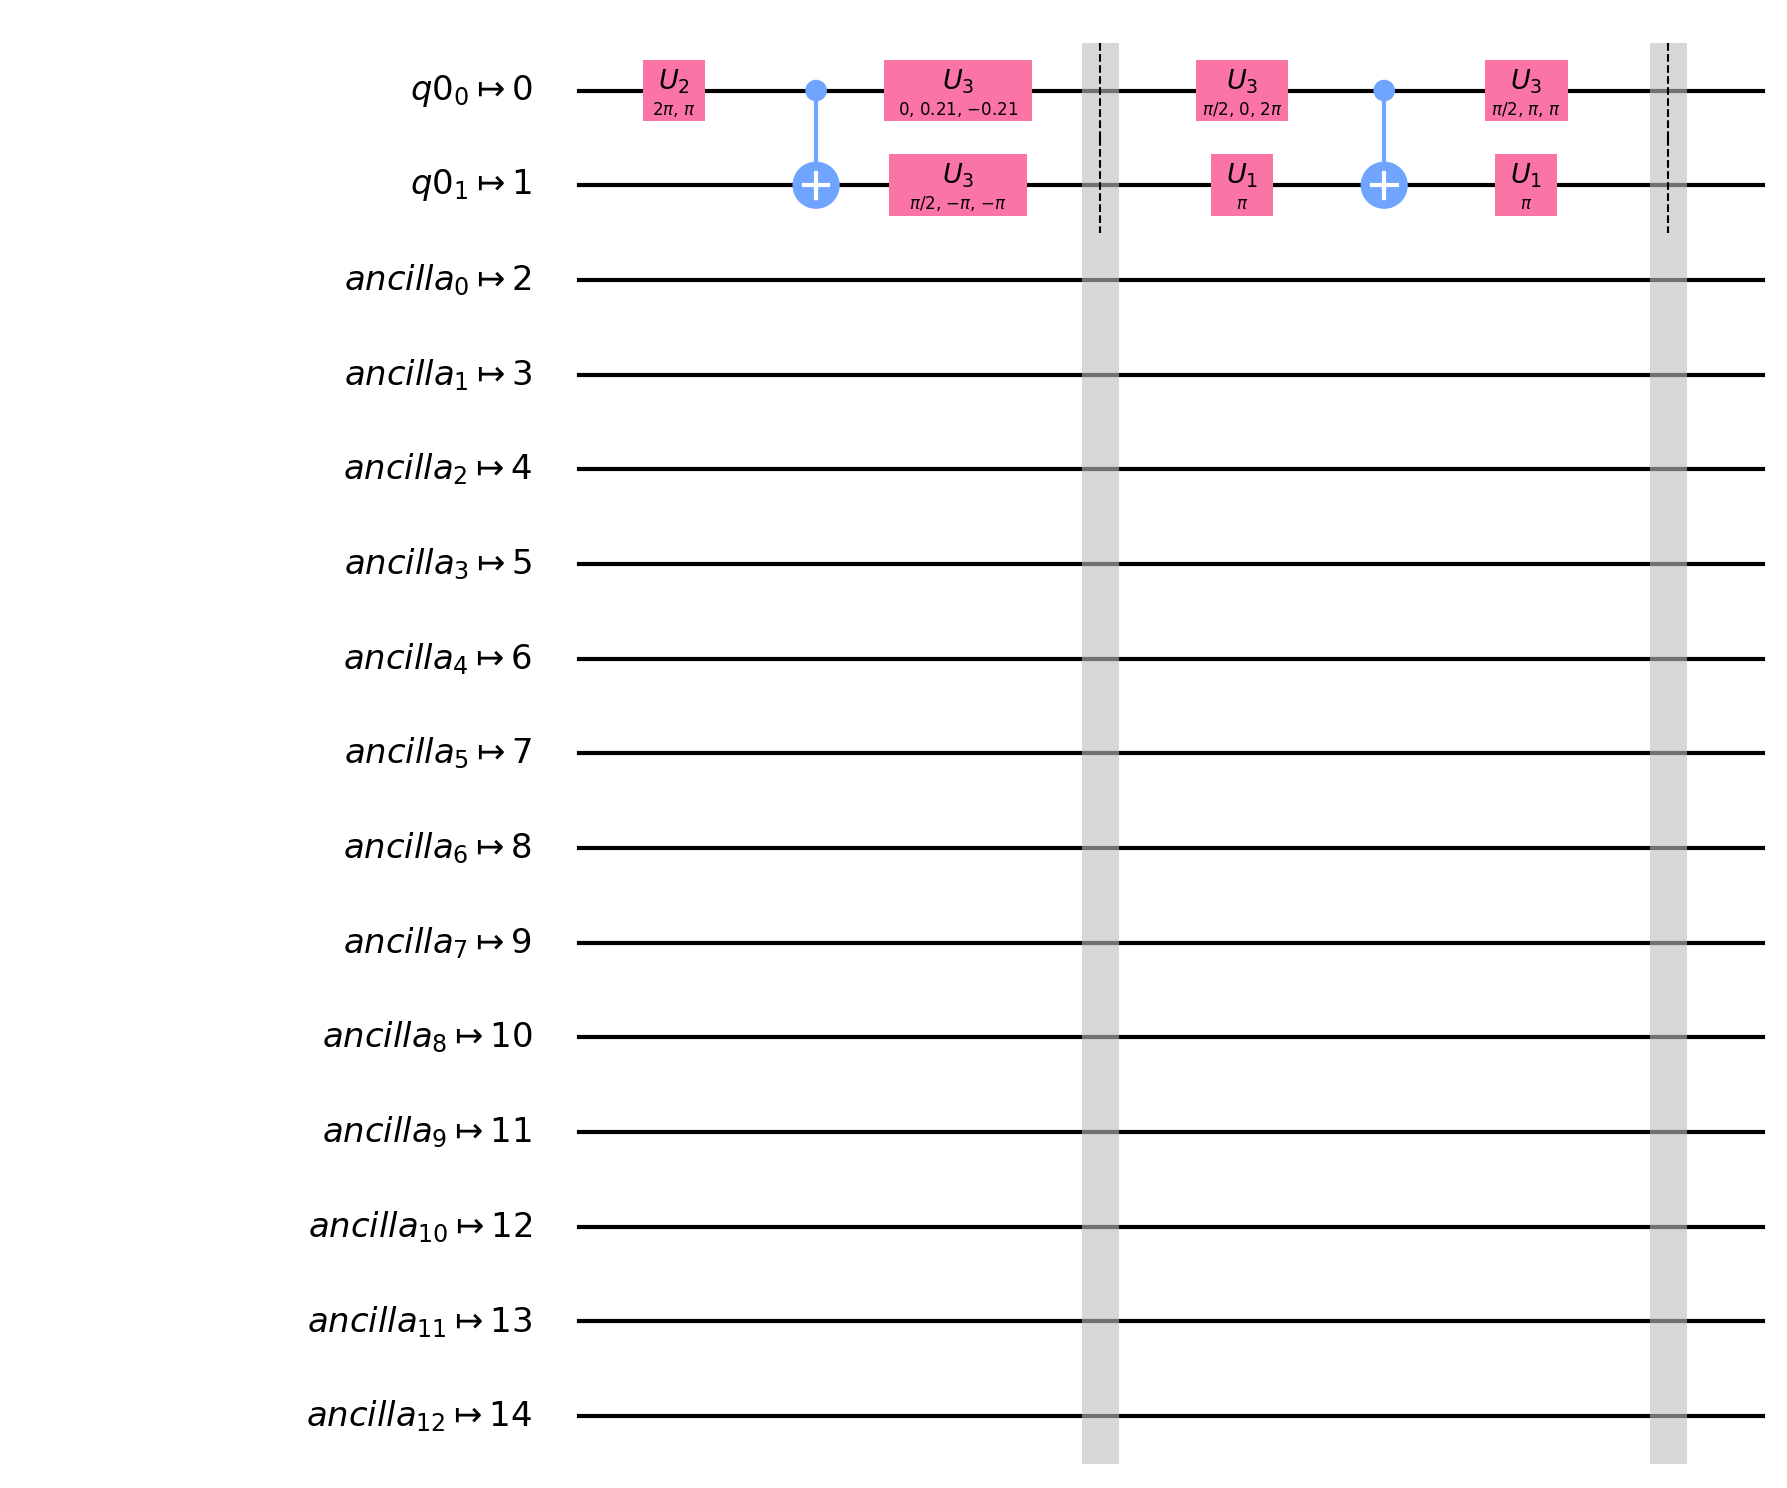
\includegraphics[width=\textwidth]{images/grover_melbourne.png}
  \caption{\textbf{Grover's Algorithm:} All backends implement Grover's
    Algorithm identically.}
  \label{fig:grov_trans}
\end{figure*}

\end{appendices}

%%% Local Variables:
%%% mode: latex
%%% TeX-master: "report"
%%% End: